\documentclass[xcolor=dvipsnames]{beamer}
\usepackage{algorithm}
\usepackage{algorithmic}
\usepackage[]{natbib}
\usepackage{alltt}
\usepackage{graphicx}

% Setup appearance:

%\usetheme{Madrid}
\usetheme{Copenhagen}
\usefonttheme[onlylarge]{structurebold}
\usecolortheme[RGB={0,63,135}]{structure} 
\setbeamercolor{normal text}{fg=Black}
\setbeamerfont*{frametitle}{size=\normalsize,series=\bfseries}
%\setbeamertemplate{navigation symbols}{}

% Standard packages

\usepackage[english]{babel}
%\usepackage[latin1]{inputenc}
%\usepackage{times}
%\usepackage[T1]{fontenc}
%\usepackage{nnfootnote}
\usepackage{amsfonts}
\usepackage{amsmath}
\usepackage{xspace}

%\newcommand{\argmax}{\operatornamewithlimits{argmax}}
\def\newblock{\hskip .11em plus .33em minus .07em}

% Author, Title, etc.

\title[YAPPL] 
{
  YAPPL\\
  Yet Another Probabilisitic\\ Programming Language \\
}


\author[Hu, Huggins, Hyttinen, \& McGrew]
{
  David~Hu\\
  Jonathan~Huggins\\
  Hans~Hyttinen\\
  Harley~McGrew\\
}

\institute[Columbia University]
{
  %\inst{1}%
  Columbia University
}

\date[December, 2011]
{December, 2011}

\begin{document}

%\nofootnotemark
\begin{frame}
  \titlepage
\end{frame}


\frame[t] {
\frametitle{Overview: Introduction}
Todo
\newline
\newline
Inspiration
\begin{itemize}
\item Church
\item HANSEI
\item OCaml
\end{itemize}
}


\frame[t] {
\frametitle{Overview: Motivations}
Todo
}

\frame[t] {
\frametitle{Tutorial 1}
Todo.
}

\begin{frame}[fragile]
\frametitle{Tutorial 2}
\begin{alltt}
~seed;
fun int:geom float:q =
  fun int:geom_helper float:orig_q int:i =
    if ~rand < orig_q then i
    else ~geom_helper orig_q (i+1)
  in 
    ~geom_helper q 1
in
\end{alltt}
\end{frame}

\begin{frame}[fragile]
\frametitle{Tutorial 3}
\begin{alltt}
fun int:try_g = ~geom 0.1 given $ > 100 in
~print_line ~try_g;
~print_line ~try_g;
~print_line ~try_g;
~print_line ~try_g;
~print_line ~try_g;

fun int:try_g2 = ~geom 0.1 given $ > 10 in
~print_line ~try_g2;
~print_line ~try_g2;
~print_line ~try_g2;
~print_line ~try_g2;
~print_line ~try_g2
\end{alltt}
\end{frame}

\frame[t] {
\frametitle{Implementation 1}
Todo\\
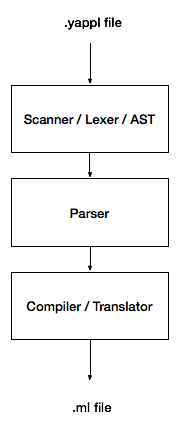
\includegraphics[scale=0.5]{block-diagram.png}
}

\begin{frame}[fragile] 
\frametitle{YAPPL code conversion to AST}
\begin{alltt} 
fun int:t1 int:a =
    a + 3
in
~print_line ~t1 2 
\end{alltt}

\end{frame}

\begin{frame}[fragile]
\frametitle{YAPPL code conversion to AST}
\begin{alltt}
FuncBindings
    FuncBind =
        FuncDecl(t1, ValType(Int), Decl(a, ValType(Int))
        Binop +
            Id a
            IntLit 3
    Eval print_line
        Eval t1
            IntLit 2
            Noexpr
        Noexpr

\end{alltt}
\end{frame}

\frame[t] {
\frametitle{Code Generation}

 {\bf Important steps}

\begin{itemize}
  \item Generate symbol table
     \begin{itemize}
        \item tracks identifiers and type
        \item can point to parent symbol table for scoping
     \end{itemize}
  \item expr\_to\_string
     \begin{itemize}
        \item main function for evaluation of ast
        \item resolves reserved identifiers before using symtable
     \end{itemize}
  \item Compile OCaml to executable
      \begin{itemize}
         \item links with builtin (includes functions like rand)
      \end{itemize}  
\end{itemize}
}

\frame[t] {
\frametitle{Summary}
\begin{itemize}
\item Yet Another Probabilisitic Programming Language, but
\begin{itemize}
\item Cleaner syntax
\item Built-in constructs: memoization, conditionals
\end{itemize}
\item \texttt{.ypl} $\rightarrow$ translation $\rightarrow$ \texttt{.ml} $\rightarrow$ execution
\begin{itemize}
\item Condensed: \texttt{./yapplc program.ypl ; ./program}
\end{itemize}
\end{itemize}
}

\frame[t] {
\frametitle{Summary}
{\bf Lessons learned}
	\begin{itemize}
	\item Start early
	\item Parallelize work structure
	\item Project scope
		\begin{itemize}
		\item Big: potential to do cool stuff
		\item Small: it will probably actually work
		\end{itemize}
	\end{itemize}
}

\end{document}
